\documentclass{beamer}
\usecolortheme{beaver}

\usepackage[utf8]{inputenc}
\usepackage[spanish]{babel}
\usepackage{graphicx}
\usepackage{hyperref}
\usebackgroundtemplate%
{%
    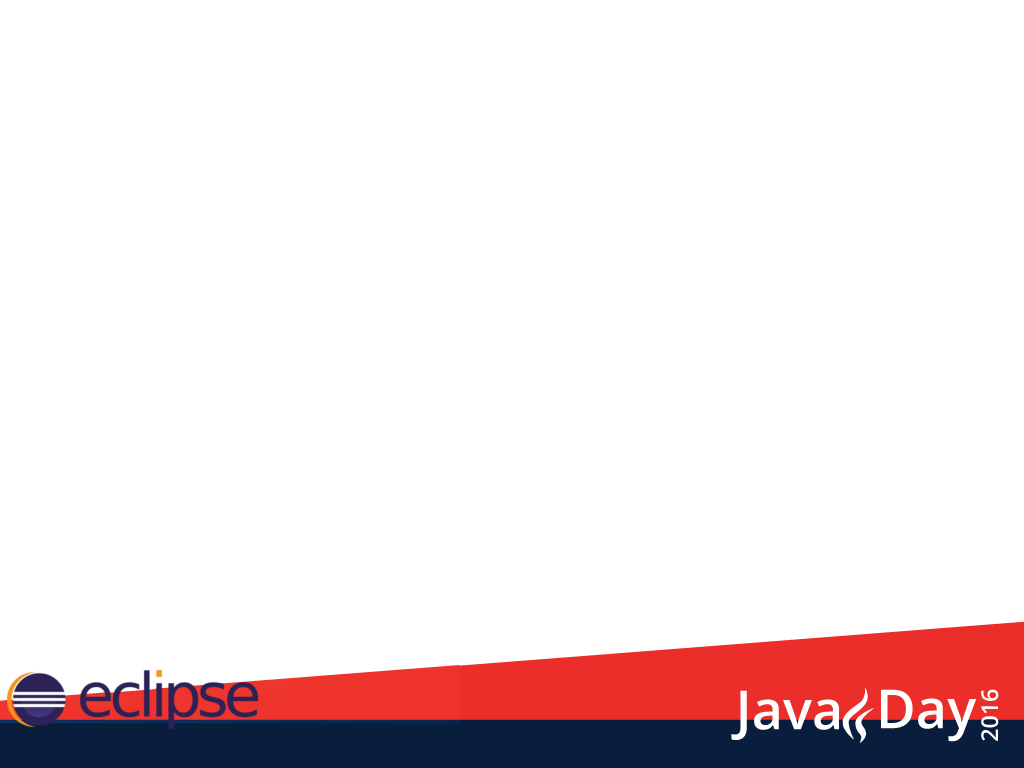
\includegraphics[width=\paperwidth]{Images/fondo}%
}

\AtBeginSection[]{
	\begin{frame}
		\vfill
		\centering
		\begin{beamercolorbox}[sep=8pt,center,shadow=true,rounded=true]{title}
			\usebeamerfont{title}\insertsectionhead\par%
		\end{beamercolorbox}
		\vfill
	\end{frame}
}

\title{Creando aplicaciones Web con JavaEE 7 y JBoss Forge}
\author{Víctor Orozco}
\institute{Nabenik}
\date{\today}

\begin{document}

\frame{\titlepage}

\section*{Intro}
\begin{frame}{Víctor Orozco}
	\begin{columns}[T] % contents are top vertically aligned
		\begin{column}[T]{5cm} % each column can also be its own environment
			\begin{itemize}
				\item Developer (JVM/Open Source Advocate)
				\item JUG Leader
				\item Consultor independiente (Nabenik)
				\item Profesor universitario
				\item \href{https://twitter.com/tuxtor}{@tuxtor}
				\item \href{https://vorozco.com}{The J*} 
			\end{itemize}
		\end{column}
		\begin{column}[T]{5cm} % alternative top-align that's better for graphics
			\begin{figure}
				\centering
				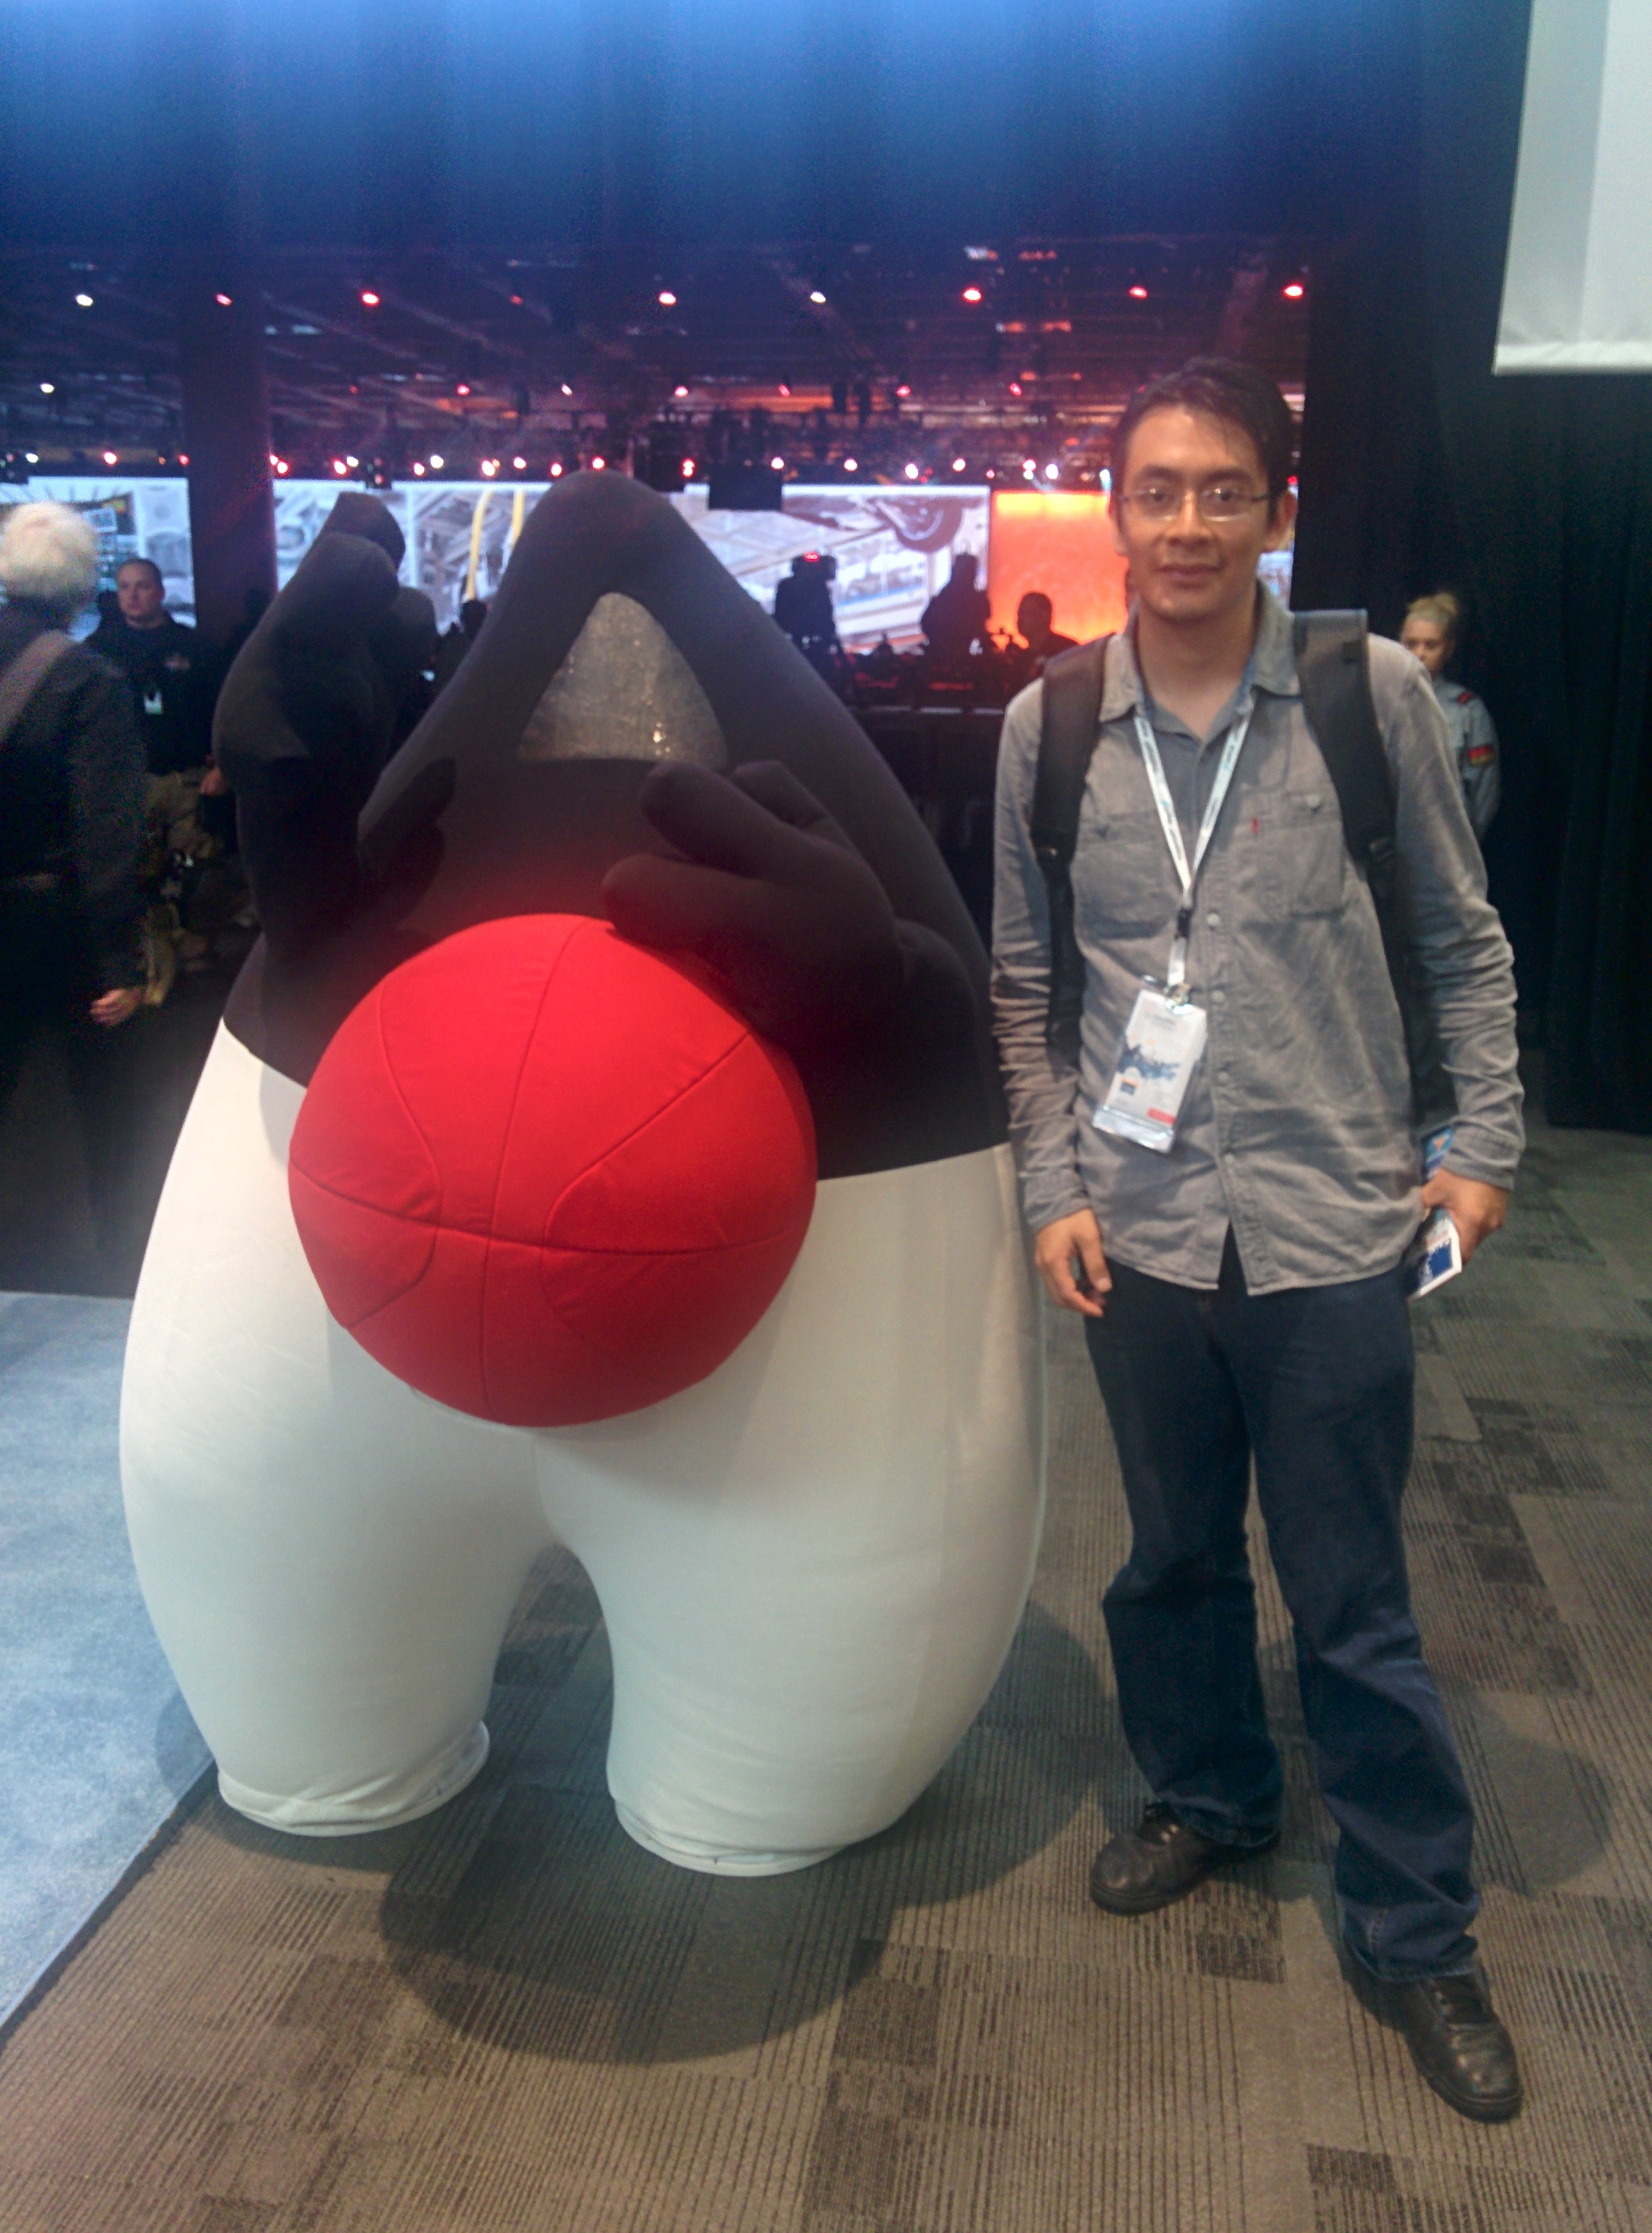
\includegraphics[width=0.7\linewidth]{Images/j1.jpg}
			\end{figure}
			
		\end{column}
	\end{columns}
\end{frame}

\section{JavaEE 7}
\begin{frame}{Framework - Ecosistema}
	\begin{figure}
		\centering
		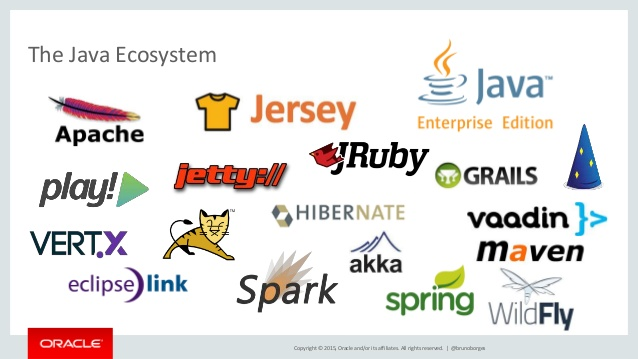
\includegraphics[width=0.9\linewidth]{Images/ecosystem}
	\end{figure}
\end{frame}

\begin{frame}{Framework - Enterprise}
	\begin{figure}
		\centering
		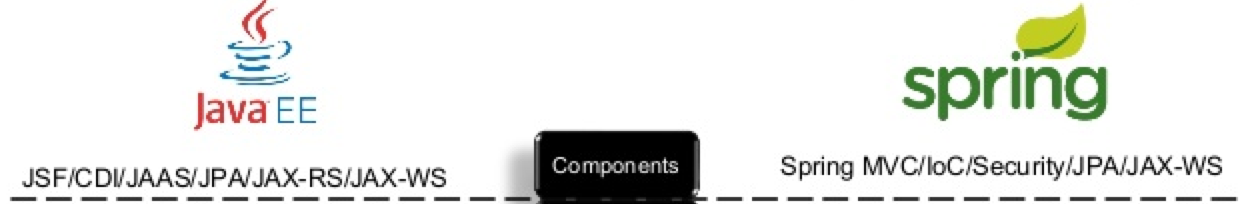
\includegraphics[width=\linewidth]{Images/javaeesp}
	\end{figure}
\end{frame}

\begin{frame}{JavaEE 7}
	\begin{figure}
		\centering
		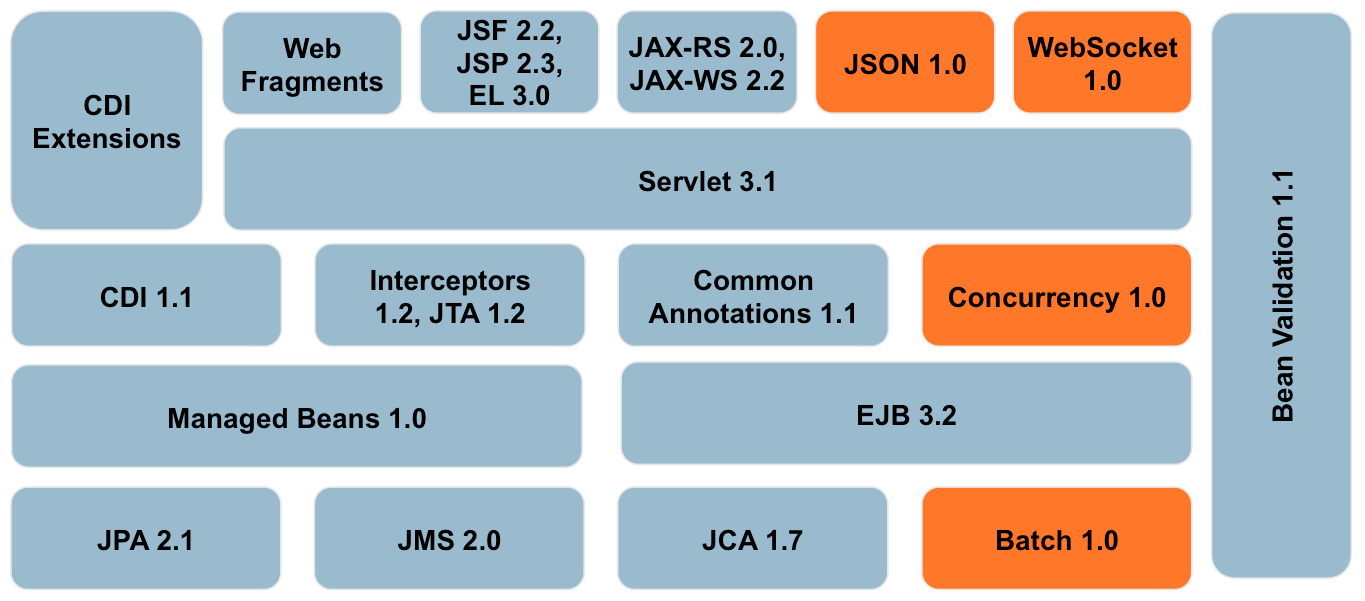
\includegraphics[width=0.9\linewidth]{Images/javaee7-pancake.png}
	\end{figure}	
\end{frame}

\begin{frame}{JavaEE 7}
	\begin{itemize}
		\item API Rest - JAX-RS 2.0
		\item WebSocket - WebSocket 1.0, Servlet 3.1
		\item JSON - JSON API 1.0
		\item SOA, Microservices
	\end{itemize}
	\begin{figure}
		\centering
		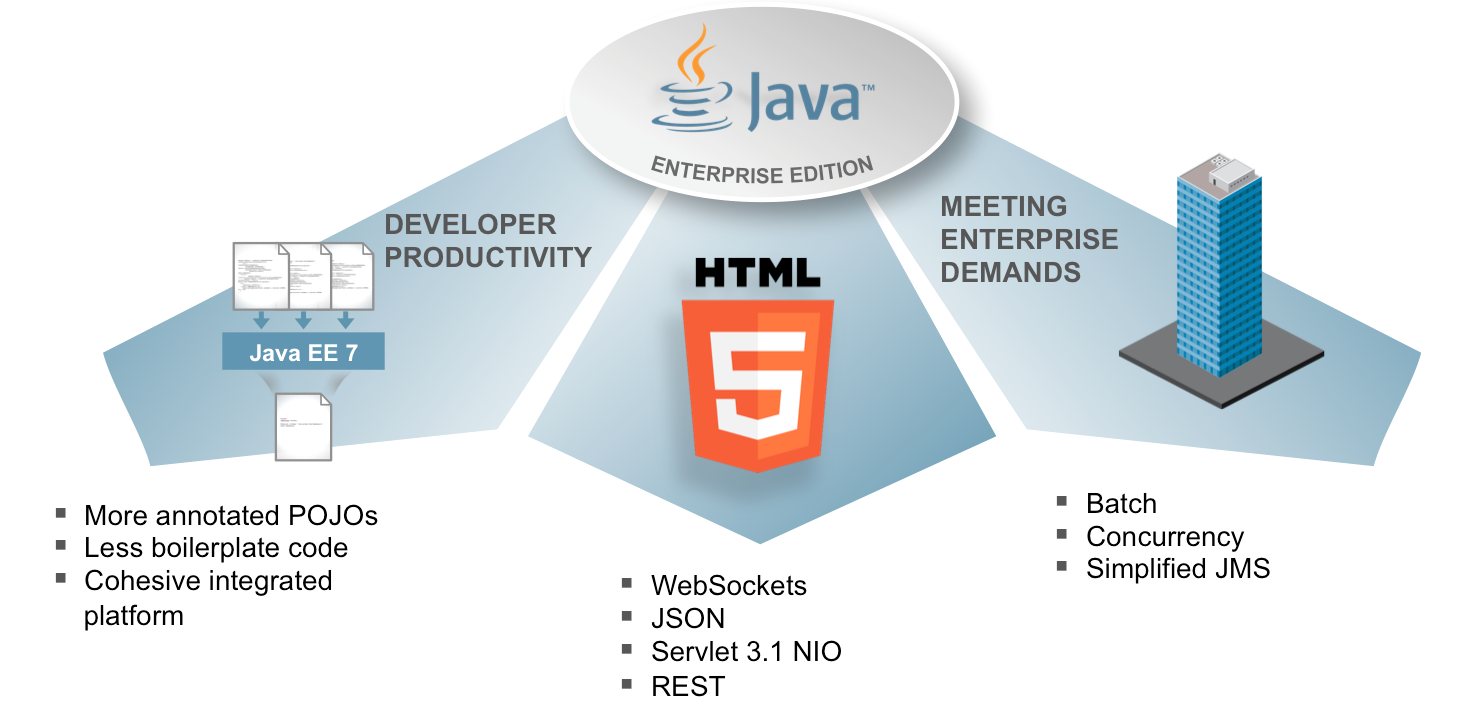
\includegraphics[width=0.65\linewidth]{Images/javaee7-theme}
	\end{figure}
\end{frame}

\section{Eclipse Neon}
\begin{frame}{Eclipse Neon}
	\begin{figure}
		\centering
		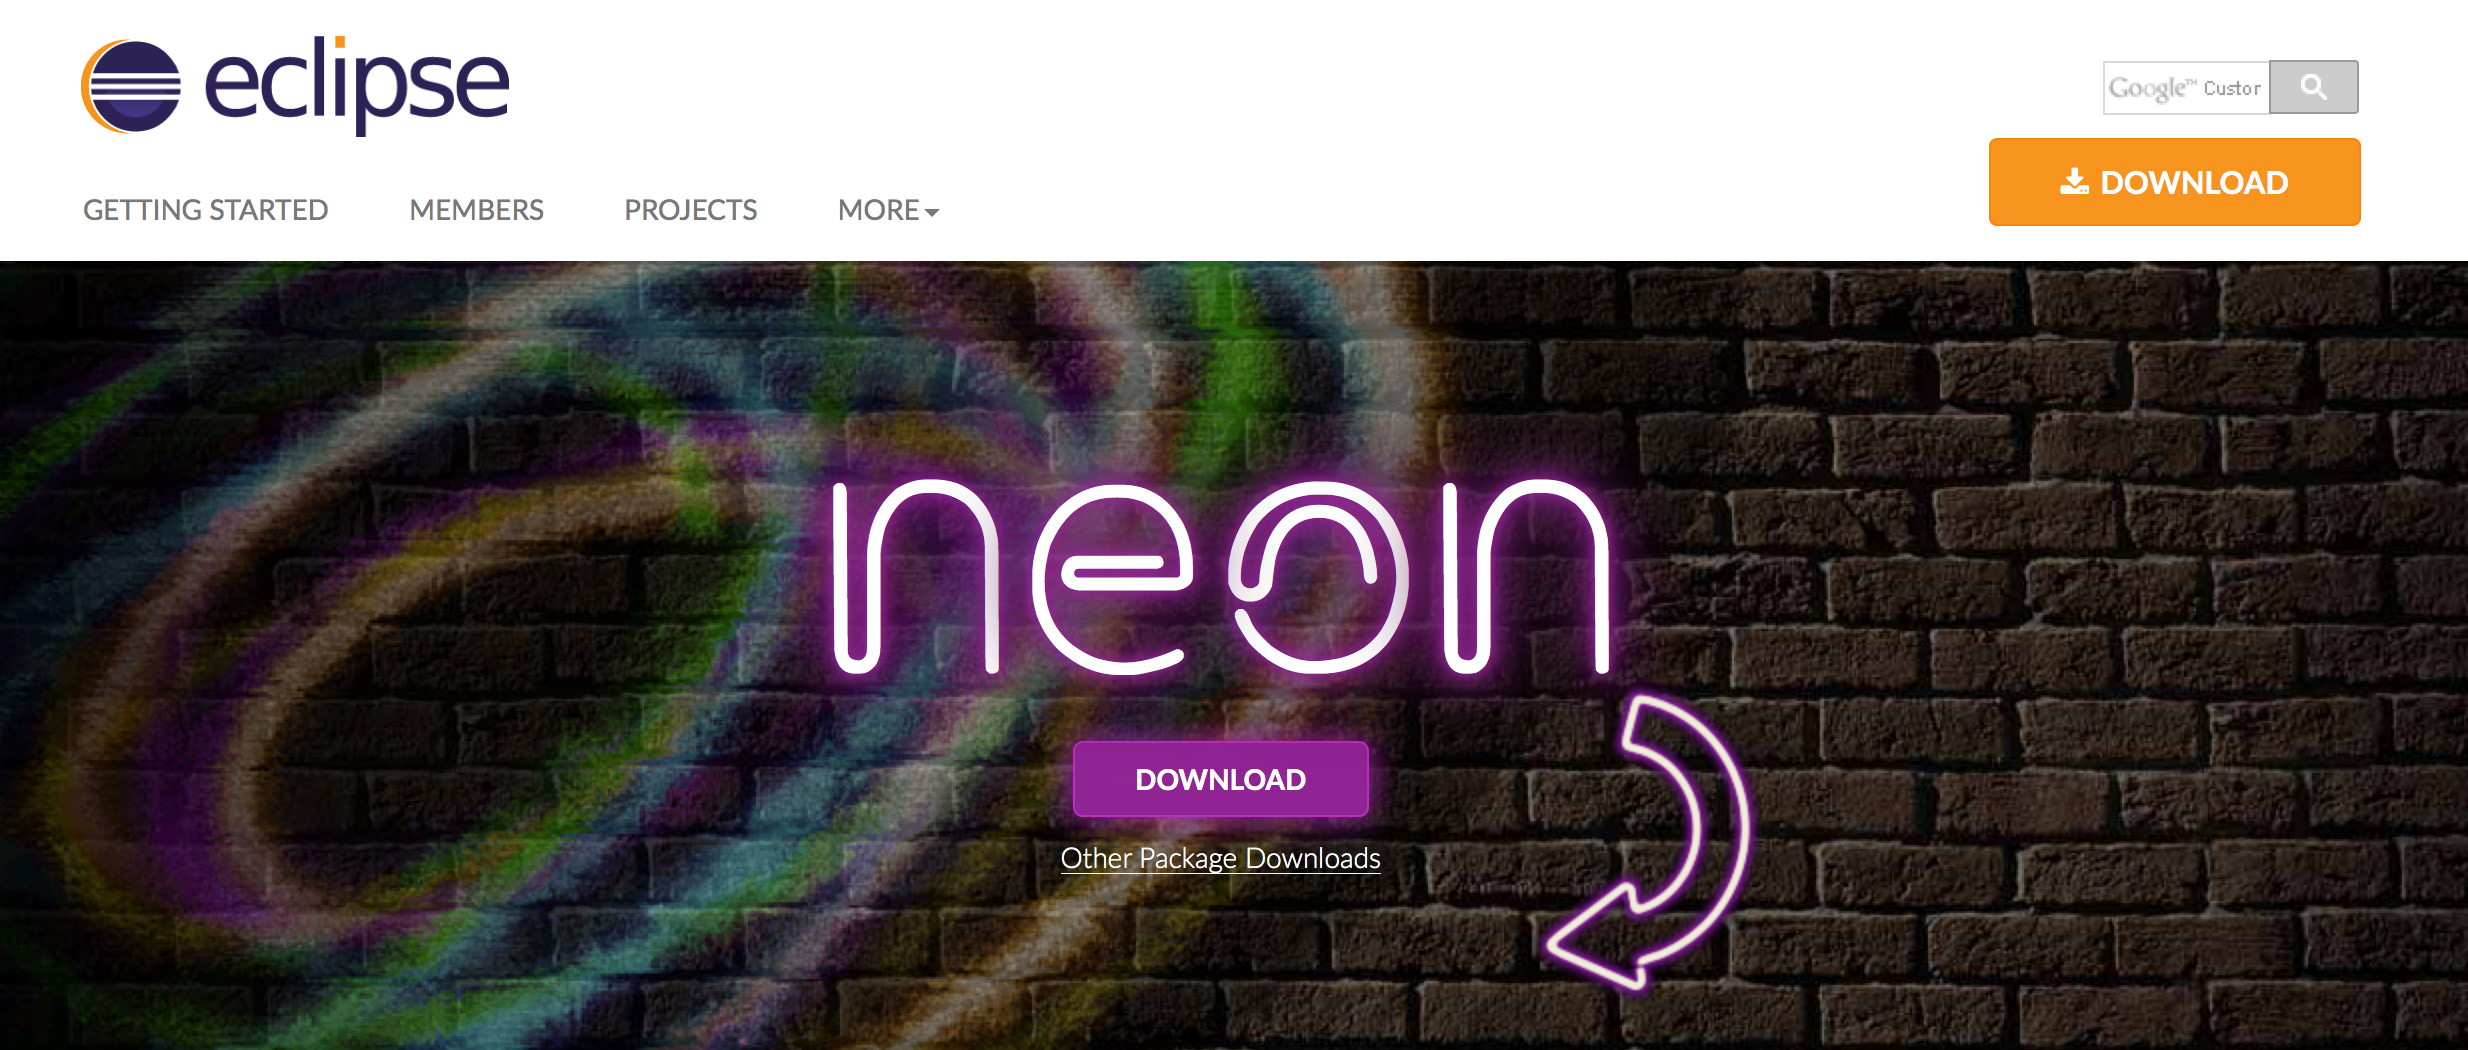
\includegraphics[width=0.90\linewidth]{Images/neon}
	\end{figure}
\end{frame}

\begin{frame}{Eclipse Neon}
	\begin{itemize}
		\item 13 años en desarrollo
		\item JSDT - JSON Editor, Grunt/Gulp, V8 Debugger
		\item HiDPI (yey!)
		\item PHP 7
		\item Cloud settings
		\item Soporte docker
		\item Gradle, EGerrit, Paho, Android Tooling, . . .
	\end{itemize}
\end{frame}

\begin{frame}{Eclipse Neon}
	En 2014 . . .
	\begin{figure}
		\centering
		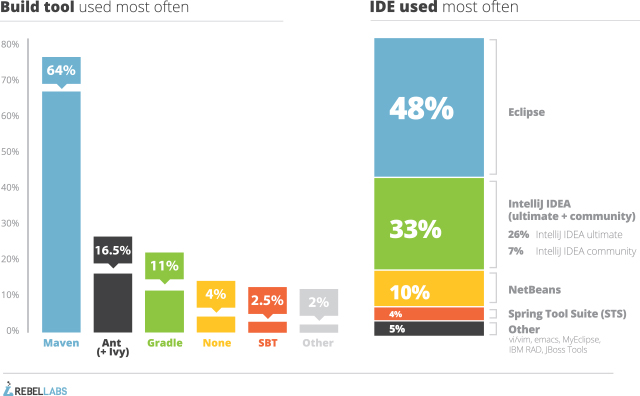
\includegraphics[width=0.9\linewidth]{Images/ide}
	\end{figure}
\end{frame}

\begin{frame}{JBoss Tools}
	\begin{figure}
		\centering
		
\includegraphics[width=0.9\linewidth]{Images/devstudio10}
	\end{figure}
\end{frame}

\begin{frame}{JBoss Tools}
	\begin{itemize}
		\item JSDT - JSON Editor, Grunt/Gulp, V8 Debugger
		\item OpenShift 3, Docker
		\item \textbf{Forge Tools}
		\item EAP 7.0 (yey!)
		\item CDI
		\item LiveReload (WildFly, JBoss)
		\item FrontEnd Tooling, BrowserSim
		\item Arquillian, AeroGear, Batch Tools
		\item Complemento o empaquetado
	\end{itemize}
\end{frame}

\begin{frame}{JBoss Tools}
	\begin{figure}
		\centering
		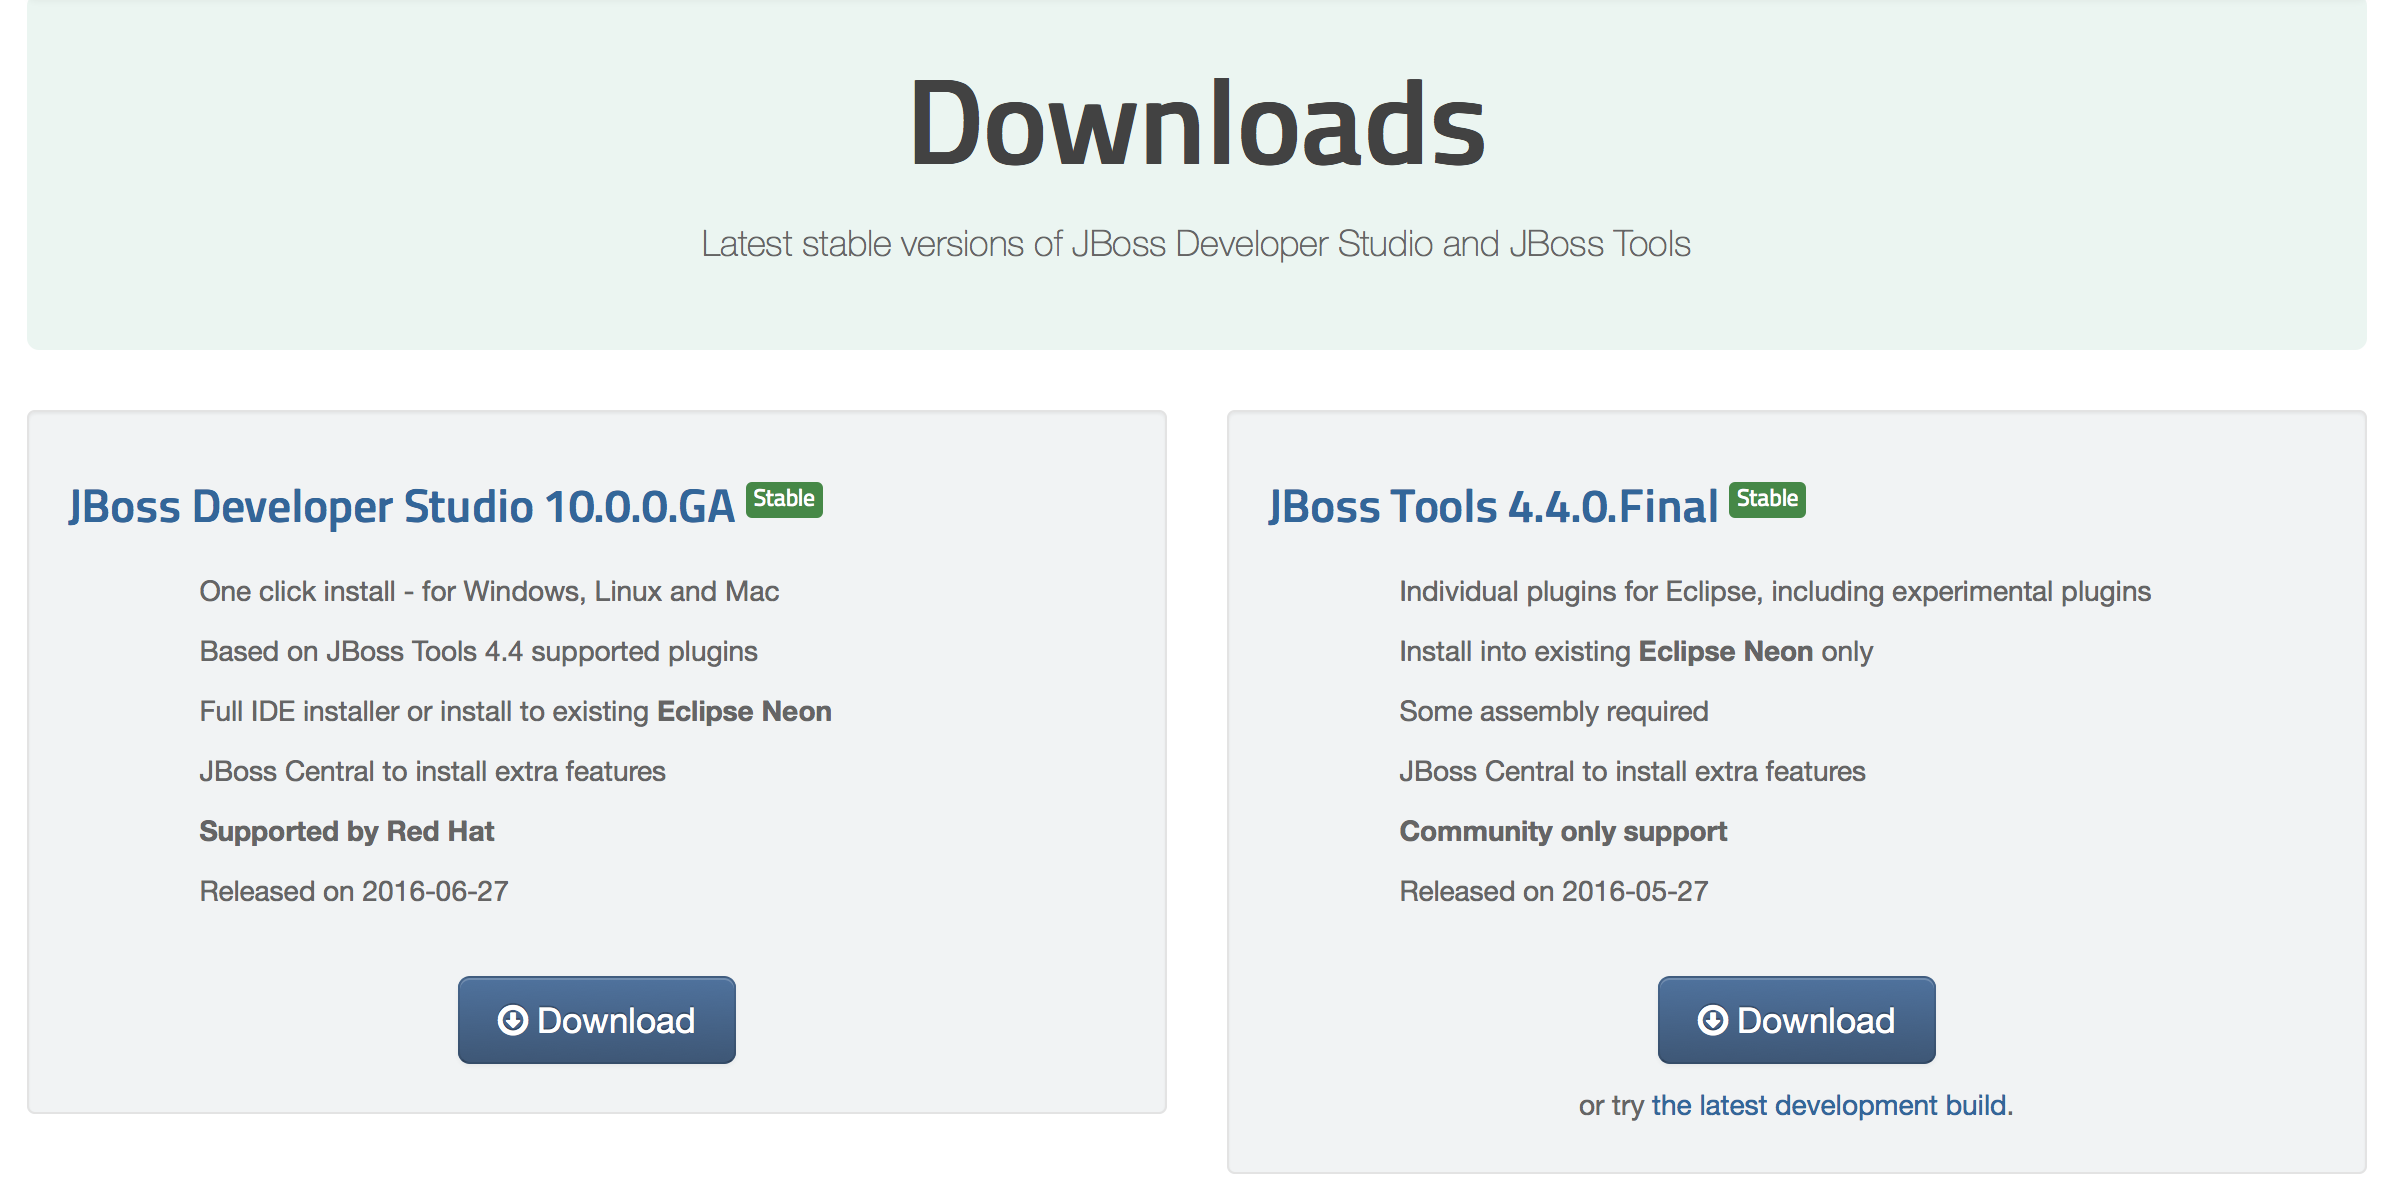
\includegraphics[width=0.9\linewidth]{Images/jtools}
	\end{figure}
\end{frame}

\begin{frame}{JBoss Forge}
	\begin{figure}
		\centering
		
\includegraphics[width=0.9\linewidth]{Images/forge}
	\end{figure}
\end{frame}

\begin{frame}{JBoss Forge}
	\begin{itemize}
		\item Layout
		\item Dependencias (pom.xml)
		\item Scaffolding
		\item Domain driven development
		\item Deployment
	\end{itemize}
\end{frame}


\section{Demo}
\begin{frame}{Arquitectura 2016}
	\begin{figure}
\centering
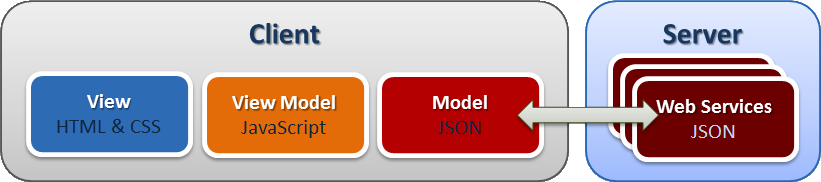
\includegraphics[width=0.9\linewidth]{Images/arq2015b}
\end{figure}
\end{frame}

\begin{frame}{JavaEE 7 - 2016}
	\begin{figure}
		\centering
		
\includegraphics[width=0.8\linewidth]{Images/anguaree.png}
	\end{figure}
\end{frame}


\begin{frame}{Ventajas}
	\begin{itemize}
		\item Existen N cantidad de bibliotecas JavaScript
		\item Independencia de backend
		\item Escalabilidad (stateless)
		\item Thin server apps
		\item Mejor tiempo de respuesta en comparación a JSF/SpringMVC
	\end{itemize}
\end{frame}

\begin{frame}{Desventajas}
	\begin{itemize}
		\item Existen n cantidad de bibliotecas JavaScript
		\item Complejidad y restricciones de REST
		\item AngularJS no sera compatible hacia atrás
	\end{itemize}
\end{frame}

\begin{frame}{Demo}
	\begin{itemize}
		\item CRUD Registro Java Day
		\item H2 + WildFly 10
		\item Bean Validation, JPA, JAX-RS, JSON
		\item AngularJS vanilla
		\item Forge Tools
		\item \url{https://github.com/tuxtor/bookstore}
	\end{itemize}
\end{frame}

\begin{frame}{QA}
	\begin{itemize}
		\item Eclipse Neon - \url{https://eclipse.org/}
		\item JBoss Tools - \url{http://tools.jboss.org/}
		\item AngularJS - \url{https://angularjs.org/}
		\item JavaEE - \url{http://docs.oracle.com/javaee/7/index.html}
		\item Libros recomendados:
		\begin{itemize}
			\item Java EE 7 Essentials - Arun Gupta
			\item Developing RESTful Services with JAX-RS 2.0 - Masoud Kalali, Bhakti Mehta
			\item Eloquent JavaScript - Marijn Haverbeke
		\end{itemize}
	\end{itemize}
\end{frame}

\begin{frame}{Gracias}
\begin{itemize}
\item me@vorozco.com
\item \url{https://www.vorozco.com}
\item \url{http://github.com/tuxtor/slides}
\end{itemize}
\begin{center}

\includegraphics[width=0.1\linewidth]{Images/cclogo}
\\
This work is licensed under a Creative Commons Attribution-ShareAlike 3.0 Guatemala License.
\end{center}
\end{frame}
\end{document}
